\section{Distributed Instantiation}
\label{sec:implementation}

We describe the realization of \name programming model on top of a persistent
distributed store and the language extensions to enable and enforce the
constraints of the \name.

\name programming model is realized on top of Irmin~\cite{irmin}, an OCaml
library database implementation that is part of the MirageOS
project~\cite{mirage}. Irmin provides a persistent multi-versioned store with
with a content-addressable heap abstraction. Simply put, content-addressability
means that the address of a data block is determined by its content. If the
content changes, then so does the address. Old content continues to be
available the old address. Content-addressability also results in constant time
structural equality checks, which we exploit in our mergeable rope
implementation (Section~\ref{sec:ropes}).

Irmin provides support for distribution, fault-tolerance and concurrency
control by incorporating Git distributed version control~\cite{git} protocol
over its object model. Indeed, Irmin is fully compatible with the Git command
line tools. Distributed replicas in \name are created by cloning a \name
repository. Due to \name's mergeable type, each replica can operate completely
independently, accepting client requests, even when disconnected from other
replicas, resulting in a fully available distributed database system.

\begin{wrapfigure}{L}{.5\textwidth}
	\begin{center}
	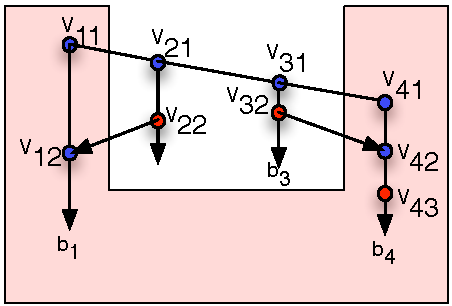
\includegraphics[scale=0.8]{Figures/partitions}
	\end{center}
  \caption{Network partitions may leave branches $b_1$ and $b_4$ in
  one partition (red background), and branches $b_2$ and $b_3$ in the
  other (yellow background). Access to full history on both sides of
  the partition lets both sides make progress.}
	\label{fig:partitions}
\end{wrapfigure}

Concurrent operations in Irmin are tracked within the notion of branches,
allowing the programmer to explicitly merge the branches on demand. \name
realizes the concurrent programming model on top of the notion of branches;
each replica operates on its own branch, and thus is isolated from actions on
other replicas. In presence of network partitions, the nodes in one partition
may not receive updates from the other partition, hence merges cannot
happen across a partition. This can be a problem if a pair of branches
in one partition (the current partition) have their loci
(Sec.~\ref{sec:meta}) in the other partition (the remote partition),
hence cannot merge. Fig.~\ref{fig:partitions} illustrate this problem
for the branching structure of
Fig.~\ref{fig:external-lcas}.

Fortunately, the access to full (causal) branching history assured by
Irmin at every node comes to the rescue. Relying on the history, the
current partition can fork-off (\C{fork}) new branches that start
where the remote branches left, and map them to new (virtual) nodes
that emulate the nodes in the remote partition. For the example in
Fig.~\ref{fig:partitions}, the partition of $b_1$ and $b_4$ can fork
new branches $b_2'$ and $b_3'$ from $b_2$ and $b_3$, respectively, and
resume the activity as if the partition never happened. The ability to
track full provenance information is thus crucial for \name to
overcome network partitions, making it an appropriate programming
model for highly-available replicated data types. \name monad conceals
the branching structure, but also transparently performs the necessary
merges to obtain a history graph with a unique lowest common ancestor.

Importantly, Irmin supports user-defined three-way merge functions for
reconciling concurrent operations. While Irmin's merge functions are defined
over objects on Irmin's content-addressable heap, \name's merge functions are
defined over OCaml types. We address this representational mis-match with the
help of OCaml's PPX metaprogramming support~\cite{ppx} to derive bi-directional
transformations between objects on OCaml and Irmin heaps. We also derive the
various serialization functions required Irmin. This address the representation
mismatch between the application and storage layers. Synchronization between
replicas is performed using Git's notion of pushing and pulling updates from
remotes over the Git transfer protocol~\cite{git-tp}. As a result, we reap the
benefits of efficient delta-transfer (only missing objects are transferred
between replicas), compression and end-to-end encrypted communication between
the replicas.
